
\section{Introduction}
Before we can begin to talk about what analysis is about, we must have a clear
notion of the objects that we want to study. Mathematics started with the study
of numbers and that's what we shall start with here. Just like driving a car
does not require knowledge of how an engine works, we will not enter into a
discussion of all properties of numbers(an interested reader might look to
\todo{more rigorous definition of numbers reference} for more information). We
must take some things for granted if we wish to get off the runway. We will
assume you to be familiar with rational, or decimal numbers such as
\begin{equation}\label{eq:numbers}
1, \qquad 2.56, \qquad \frac{1}{3}, \qquad 0.347
\end{equation}

This set of numbers is great for many purposes, including almost everything in
our day to day life, but we can show it isn't quite satisfactory for all
purposes. Take, for example, the following triangle.

\begin{figure}\label{fig:right-triangle}
    \centering
    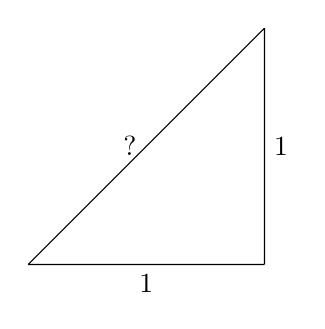
\begin{tikzpicture}
    \draw (0,0)  -- (3,0) node[midway, below]{1}
        (3,0) -- (3,3) node[midway, right]{1}
        (3,3) -- (0,0) node[midway, left]{?};
    \end{tikzpicture}
    \caption{Simple Right Triangle with Side Length 1}
\end{figure}

Suppose we want to figure out how long the side is labelled by ``?''. Well, if
we use the Pythagorean Theorem\marginnote{This simply says that if we have a
right triangle with sides of length $a$ and $b$, then the hypotenuse $c$ is
related to those numbers by $c^2 = a^2 + b^2$.} then we can write the following
equation. We use the letter $x$ to denote the length of the hypotenuse that we
are interested in. 

\begin{align}
    x^2 & = 1^2 + 1^2 \nonumber \\
    x^2 & = 2 \label{eq:sqrt2}
\end{align}

If the rational numbers are ``enough''\marginnote{meaning they represent
everything we can construct geometrically}, then we should be able to write $x$
as $\frac{n}{m}$ where $n$ and $m$ are integers ({$\{\ldots, -2, -1,
0, 1, 2, \ldots\}$})\todo{say rational numbers are fractions before this part}.
However, as we will see in Example \ref{ex:gaps}, this may not be the case.

\begin{example}[Existence of Gaps]\label{ex:gaps}
In this example we will set out to show that Equation \ref{eq:sqrt2} has no
solutions that are rational. To show this we will employ a method known as
proof by contradiction. We will assume that $x$ can be written as a fraction.
\begin{equation}\label{eq:sqrt2-is-rational}
    x = \frac{n}{m}
\end{equation}
We take the fraction to be as reduced as possible\marginnote{meaning we
wouldn't have something like $\frac{5}{15}$ because that can be reduced further
to $\frac{1}{3}$} and hence $n$ and $m$ are \emph{not both} even. We can plug
this into Equation \ref{eq:sqrt2} to obtain
\begin{equation*}
x^2 = \frac{n^2}{m^2} = 2 \overset{\text{multiply by } m^2}{\implies} n^2 =
2m^2
\end{equation*}
\end{example}












\section{Ordered Sets}


\section{Fields}


\section{The Real Field}


\section{The Extended Real Number System}


\section{The Complex Field}


\section{Euclidean Spaces}


\section{Appendix}


\section{Exercises}

